\section{文件组织}

\subsection{文件组织}

数据库以文件集合的形式存储.

每个文件是一系列记录.

一条记录是一系列字段.

两种记录:

\begin{itemize}
    \item 定长记录.
    \item 可变长度记录.
\end{itemize}

\subsection{定长记录}

优点:方法简单:

\begin{itemize}
    \item 从字节$n*(i-1)$开始存储记录$i$,其中$n$是每条记录的大小.
    \item 记录访问简单,但记录可能跨块.
    \item 修改:不允许记录跨越块边界
\end{itemize}

删除记录$i$:可选方法:

\begin{itemize}
    \item 方法1:将记录$i+1,...,n$移动到$i,...,n-1$
    \item 方法2:将记录$n$移动到$i$
    \item 方法3:不移动记录,但将所有空闲记录链接到空闲列表上
\end{itemize}

\subsection{空闲列表}

将文件头中第一个已删除记录的地址存储(还有其它信息).

使用第一条记录来存储第二条已删除记录的地址,以此类推.

可以将这些存储的地址视为指针,因为它们"指向"记录的位置.

3个优势:更多空间高效表示:复用普通空间免费记录的属性用于存储指针.(无存储在使用中的指针记录)

\subsection{可变长度记录}

可变长度记录在数据库系统中有多种产生方式:

\begin{itemize}
    \item 在文件中存储多种记录类型
    \item 允许一个或多个字段(如字符串(varchar))具有可变长度的记录类型
    \item 允许重复字段的记录类型(在一些旧的数据模型中使用)
\end{itemize}

属性按顺序存储.

由固定大小(偏移量/长度)表示的可变长度属性,实际数据存储在所有固定长度属性之后

由空值位图表示对空值.

\subsection{槽页结构}

\begin{figure}[H]
    \centering
    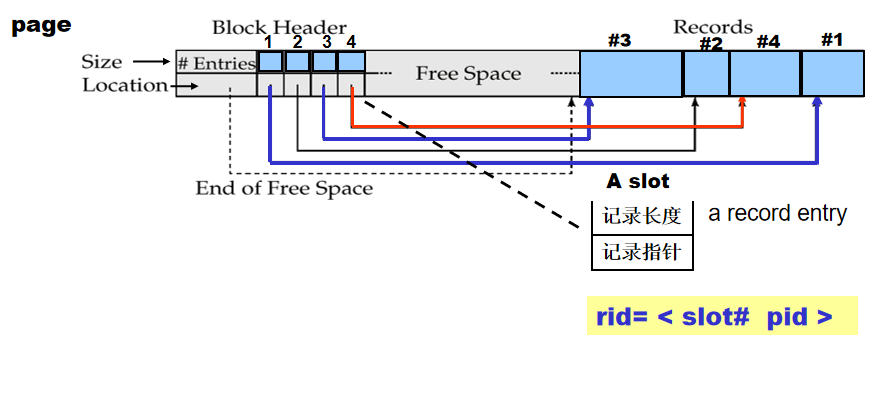
\includegraphics[width=0.8\linewidth]{image8.png}
    \caption{Slotted Page Structure}
    \label{}
\end{figure}

rid = <slot\# pid>

槽式页面头部包含:

\begin{itemize}
    \item 记录条目数量
    \item 块中可用空间结束
    \item 每条记录的位置和大小
\end{itemize}

记录可以在页面内移动,以保持它们连续且彼此之间没有空白空间;必须更新头部中的条目.(页内无碎块;删除时页内移动记录)

指针(索引)不应直接指向记录---相反,它们应指向头部中记录的条目---间接指针


\subsection{定长表示}

定长表示:预留空间,指针

预留空间:可以使用已知最大长度的定长记录;较短记录中的未使用空间用空字符或记录结束符号填充.

\subsection{指针方法}

可变长度记录由一系列固定长度记录表示,这些记录通过指针链接在一起.

即使不知道最大记录长度也可以使用.

指针结构的缺点:除了链中的第一条记录外,所有记录都会浪费(用于分支名称的)空间.

解决方案是允许文件中有两种块:

\begin{itemize}
    \item 锚块:包含链的第一条记录
    \item 溢出块:包含除链的第一条记录外的其它记录.
\end{itemize}